\documentclass[sigconf]{acmart}

\usepackage{graphicx}
\usepackage{algorithm} % for algorithms
\usepackage{algpseudocode}
\usepackage{booktabs} % For formal tables
\usepackage{amsthm} % For claims
\usepackage{bbm} % indicator function

% table
\usepackage[flushleft]{threeparttable} % http://ctan.org/pkg/threeparttable
\usepackage{booktabs,caption}

\theoremstyle{remark}

\settopmatter{printacmref=false, printccs=true, printfolios=true}
\pagestyle{empty} % removes running headers

\newcommand{\PicScale}{0.5}
\newcommand {\FlameStream} {FlameStream}
\begin{document}

\copyrightyear{2019} 
\acmYear{2019} 
\setcopyright{acmcopyright}
% \acmConference[BeyondMR'18]{Algorithms and Systems for MapReduce and Beyond }{June 15, 2018}{Houston, TX, USA}
% \acmBooktitle{BeyondMR'18: Algorithms and Systems for MapReduce and Beyond , June 15, 2018, Houston, TX, USA}
% \acmPrice{15.00}
% \acmDOI{10.1145/3206333.3209273}
% \acmISBN{978-1-4503-5703-6/18/06}

\title {Distributed classification of text streams: challenges and limitations}

\author{Artem Trofimov,$^ {1}$    Mikhail Shavkunov,$^2$    Sergey Reznick,$^3$     Nikita Sokolov,$^{4}$   Mikhail Yutman,$^2$ \\   Igor E. Kuralenok,$^1$    and  Boris Novikov$^ {2}$ }
\affiliation{%
\institution{$^1$JetBrains Research}
}
\affiliation{%
\institution{$^2$National Research University Higher School of Economics}
}
\affiliation{%
\institution{$^3$ Kofax}
}
\affiliation{%
\institution{$^4$ ITMO University}
  \city{St. Petersburg} 
  \country{Russia}
}
\email{\string{trofimov9artem, ikuralenok\string}@gmail.com, borisnov@acm.org}

\begin{abstract}

Distributed stream processing engines seem as suitable platforms for large-scale text classification with low latency requirements. However, this straightforward approach has important pitfalls that are easy to miss. In this work, we emphasize the challenges that a developer of text stream classification pipeline face and propose a data flow on top of~\FlameStream\ processing engine that is able to overcome most of the issues. We demonstrate the feasibility of the proposed solution with a series of experiments on a stream of real-world news articles.

\end{abstract}

% \keywords{Data streams, exactly-once, drifting state, optimistic OOP}

\maketitle

\thispagestyle{empty}

\section {Introduction}
\label {fs-short-intro}

Classification of large text streams is hard, but important task for researchers and practitioners. It has a wide range of applications including detection of emerging news and current user interests, suspicious traffic analysis, spam filtering, etc. Popular open-source libraries like sklearn~\cite{sklearn_api} and NLTK~\cite{bird2009natural} provide a rich set of tools, but they mostly aim at handling static datasets. The lack of scalability across multiple computational units is another limitation of these solutions. There are plenty of works which adapt batch processing systems for text classification~\cite{semberecki2016distributed, svyatkovskiy2016large, baltas2016apache}. Their advantages are fault tolerance, high throughput, and scalability. On the other hand, these systems do not provide low latency that is a strong requirement for most streaming applications.

An immediate idea is to employ a distributed stream processing engine such as Flink~\cite{Carbone:2017:SMA:3137765.3137777} or Storm~\cite{apache:storm}. However, stream processing systems have several important differences in comparison with batch engines: 

\begin{itemize}
    \item In a general case, failure and recovery are not transparent for a user. The guarantees on data in case of failures are defined in terms of delivery guarantees: {\em at least once} and {\em exactly once}. The choice of a guarantee may affect the correctness of text classification.
    \item Most of streaming systems are inherently non-deterministic. It means that different runs on the same data may produce different results. This feature can influence the classification process as well.
\end{itemize}

In this work, we investigate the applicability of state-of-the-art stream processing systems to the text classification and demonstrate the challenges that a developer can experience. Our study reveals issues similar to the problems mentioned by TFX project team~\cite{Baylor:2017:TTP:3097983.3098021} on machine learning at scale in general: reproducibility, reliability of results, fault tolerance, etc. For demonstration, we adapt text classification data flow that is typical for batch processing systems for state-of-the-art stream processing engine Apache Flink~\cite{Carbone:2017:SMA:3137765.3137777}. We show that failures within {\em at least once} guarantee may significantly shift the distribution of classification results. It is also indicated that races due to asynchronous channels in the data flow lead to a non-reproducible outcome. We demonstrate that straightforward solutions to the revealed issues may lead to performance overhead. More sophisticated approaches to solve the problems are touched upon.

The rest of the paper is structured as follows: the problem of text classification using stream processing engines and the typical data flow are discussed in section~\ref{fs-framework}, section~\ref{fs-discussion} contains the evaluation of the data flow on top of state-of-the-art stream processing system, approaches to get around the revealed issues are introduced in section~\ref{fs-solution}, prior works on the topic are mentioned in section~\ref{fs-related}, we discuss the results and our plans in~\ref{fs-conclusion}.

\section {Classifying text streams}


Our task is to design a framework for end-to-end text streams multi-classification that is able to overcome the challenges mentioned above. We assume that there are two types of input stream elements: labeled and unlabeled texts. Every text its unique identificator. The framework should predict and deliver labels for raw texts, while labeled ones must be used for additional training. In section~\ref{DSP}, we introduce a processing engine used for computations and explain the rationale behind the choice. Data flow and its properties are explained in detail in~\ref{DF}. We touch upon the ML model that can be applied to the task in~\ref{ML}.

\subsection{Distributed stream processing\label{DSP}}

In order to process high-velocity data at scale, the stream processing systems are commonly used as a solution. The examples of such systems are Apache Flink~\cite{Carbone:2017:SMA:3137765.3137777}, Google's MillWheel~\cite{Akidau:2013:MFS:2536222.2536229}, Spark Streaming~\cite{Zaharia:2012:DSE:2342763.2342773}, and Apache Storm~\cite{apache:storm}. In these systems, every piece of data enters and exits the system one by one or within small-sized blocks. Inside a system, elements are also transformed independently from each other or with slight buffering, e.g. within time windows. Unlike batch-processing systems, the next processing stages do not wait until previous ones are completed. 

For scalability, these systems are running on clusters of computers. Calculations are evenly distributed among all computers. Usually, each operation in streaming systems has a balancing function for determining the shard, where further transformations will be done with each element. The function can be set by a user. That is, after each transformation every element can be sent to another machine using this scheme. For example, for distributed IDF processing the function should send the same words to the same shard.

Such computational model provides low latency between an input element arrival and the delivery of results, however, it is hard to provide consistency guarantees on data in case of failures. Most of the stream processing systems have a lack of determinism, which means that the result of computing is not the same between independent launches. Hence, it is challenging to create a stable framework with testing and validating final results as it was discussed in \cite{stonebraker20058} Rule 4. Another issue is connected with the exactly-once delivery guarantee. This guarantee ensures processing of each element by exactly one time. Batch-processing systems provide full fault tolerance and consistency, however in stream processing exactly-once is a challenging problem that solved with big overhead. This affects the latency and makes it less than one second which is commonly unacceptable.

In this work, our computations based on FlameStream \cite{kuralenok2018flamestream} distributed engine, which provides the following advantages:

\textbf{Determinism.} FlameStream results are determined only by input and remain the same between independent runs.

\textbf{Exactly-once.} FlameStream process data in an exactly-once manner by default, which the same data processing on the Spark systems, for example, will be at a worse performance.

The mentioned problems are solved in FlameStream with almost no overhead. This allows us to create a classifier with predictable results and due to the exactly-once delivery guarantee provide low latency.

\subsection{Data flow \label{DF}}

\subsubsection{Computational pipeline}

Similar to other stream processing systems, FlameStream sets scheme of calculations by a logical directed graph. Every vertex in the graph represents a transform operation. An oriented edge indicates the flow and kind of data.

\begin{figure}[htbp]
  \centering
  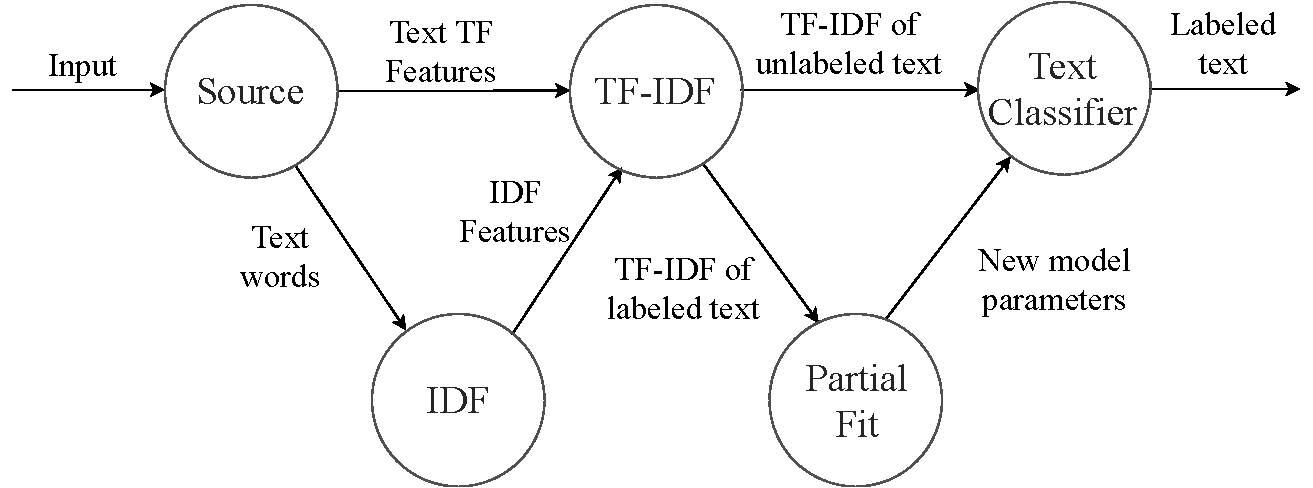
\includegraphics[scale=0.48]{pics/logical-graph}
  \caption{The logical pipeline}
  \label {logical_graph}
\end{figure}

For our task, the calculations can be illustrated as a logical graph illustrated in Figure~\ref{logical_graph}. Input vertex receives incoming texts, calculates term frequencies and transfers them to the TF-IDF vertex. It also sends words from the text to IDF vertex. IDF computes the inverse frequency of the words and delivers them to the TF-IDF vertex. TF-IDF joins corresponding inverse documents frequencies together with term frequencies within a given text. After that, the complete TF-IDF features are sent to Text Classifier vertex. Classifier predicts the label and delivers the result to the user.

\begin{figure}[htbp]
  \centering
  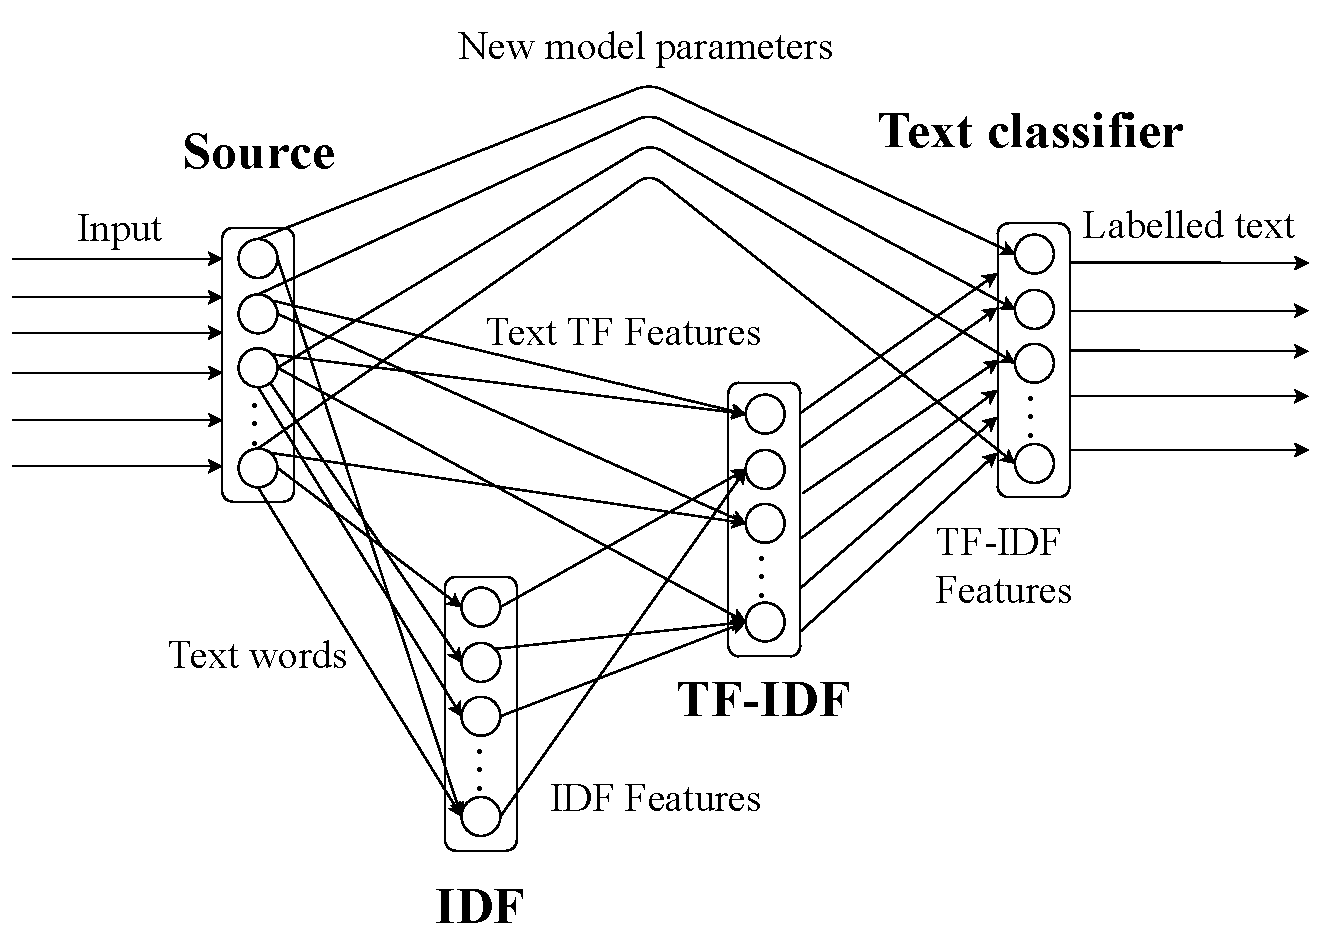
\includegraphics[scale=0.375]{pics/physical-graph}
  \caption{The physical pipeline}
  \label {physical_graph}
\end{figure}

When the pipeline is deployed, the logical graph maps into a physical graph(Figure ~\ref{physical_graph}). Each logical task is mapped to a number of physical tasks. This is, every vertex here is a single computational unit. Each rectangle denotes the same cluster of computers.

Input texts are received by all machines. Shuffle before IDF vertex are defined by a hash function of a word. Partitioning before TF-IDF physical vertices are determined by a text id. There is no network shuffle between TF-IDF and Text Classifier vertices, so they are simply chained. The partial Fit operation is located on a single machine and broadcasts model parameters to Classifier vertices.

%That is, real calculations are defined by the physical graph and can be described as follows. Input text can be received by any machine. Then Text Document vertex produces a list of words for the text and the list is distributed among all shards using the described scheme. In case of words with a high frequency such as conjunctions or prepositions, we add to them salt to the end thereby spreading all the words between the shards evenly. After that, a list of words distributed among all shards for IDF processing using the technique. In the TF-IDF stage, IDF features of the same document accumulate on a particular shard using the scheme. In the IDF and TF-IDF stages the same sharding method is used, however, the difference is during IDF processing sharding is done by a word and during TF-IDF -- by a text document. Accumulated IDF features join with the corresponding TF features. In the Text Classifier stage, classifier obtains a label for the text and returns it to the user. During this stage, the classifying process is done on the same machine, where TF-IDF features were gathered together.

\subsubsection{Dealing with concept drift}

Concept drift is a phenomenon of changing users' interests from time to time, which usually depends on recent events, and results in shifting the distribution of text classes to particular ones. Essentially, this may affect the correctness of the pipeline, more specifically, the computing of the IDF features. To overcome the issue, we use windowed IDF calculation: concrete IDF values will be provided based on input within a time window. For instance, the window can be set to a day or a week. This scheme allows us to deal with sudden changes in the topics. Similar approaches are applied in [?].

\subsubsection{Partial fit}

Figures ~\ref{logical_graph}, ~\ref{physical_graph} provide a scheme for a partial fitting. Labeled input documents accumulate in the Partial Fit vertex. Additional training is triggered by a special element, which is submitted to the input as an ordinary element. However, this element is not processed as a text and the vertices just push the element further. This process is similar to punctuation processing \cite{tucker2003exploiting}. The conditions, when the partial fitting starts, can be chosen arbitrarily by a system administrator. For example, one can update machine learning model on every 1000 labeled documents.

\subsection{ML model \label{ML}}

The classifier's model can be chosen independently from other computations. In our case, we use Multinomial Logistic Regression. At the start of the system, the initial classifier parameters such as weights can be provided by a pre-train process.

Every time, when the Partial Fit is triggered, the following process occurs, which can be described in terms of the optimization of a cost function. This function in our case is written below:

\begin{center}

$$ J(W) = -\frac{1}{m} \sum \limits_{i = 1}^{m} \sum \limits_{j = 1}^{k} \mathbbm{1}_{\left\{y^{(i)} == j\right\}} \cdot \log \frac{\exp\left({W_{j}^Tx^{(i)}}\right) }{\sum \limits_{l = 1}^{k}  \exp\left({W_{l}^Tx^{(i)}}\right) }$$ 
 $$ +  \lambda_1 ||W||_1 + \lambda_2 ||W - W_{prev}||_2 $$

\end{center} 

The number of points in a new dataset is denoted as $m$. The point with index $i$ showed as $x^{(i)}$. The number of classes is $k$. New weights are designated as $W$. The weights, that computed in the previous step, are $W_{prev}$. At the first time of triggering the process, $W_{prev}$ are the pre-trained weights. 

The formula provides the goal of the training. The first component is the standard softmax function for multiple classes. The second component keeps the l1 regularization of the weights. The important aspect is the regularization provides sparsity, hence, the model has a small size -- about 15 Mb, which can be stored and updated with low cost. To use the previous history of the classifier weights we apply l2 regularization as the third component. Fitting new points and the consideration of the previous weights ensure better accuracy of the classifier.

We are interested in finding such $W$ that minimizes $J(W)$. Taking derivatives, one can show that the gradient for each class component is:

\begin{center}

$$ \nabla_{W_j} \; J(W) = -\frac{1}{m} \sum \limits_{i = 1}^{m} \left[ x^{(i)} \left( \mathbbm{1}_{\left\{y^{(i)} == j\right\} } - \frac{\exp\left({W_{j}^Tx^{(i)}}\right)}{\sum \limits_{l = 1}^{k}  \exp\left({W_{l}^Tx^{(i)}}\right)} \right) \right] $$
$$ - \; \lambda_1 sign\left(W\right) - \frac{\lambda_2}{2} \left(W - W_{prev} \right), \; j = [1..k] $$

\end{center} 

We use Stochastic Gradient Descent for optimization. In experiments ~\ref{fs-short-experiments} section, model performance is presented.

\section {Experiments}
\label {fs-experiments}

To prove the feasibility of the proposed framework we conducted a series of experiments. We show the efficiency and scalability of the distributed streaming dataflow on the top of~\FlameStream\ processing system. Latency and throughput are used as performance metrics. We also demonstrate achieved accuracy using a simple machine learning model. As a dataset, we used an open corpus of news articles from Russian media resource lenta.ru~\cite{lentaru}. This dataset contains about 700 000 documents, which are labeled by one of 90 different topics. In the experiments, we generated a stream consisted of articles from the dataset sorted by the time of publishing.

\begin{figure}[htbp]
  \centering
  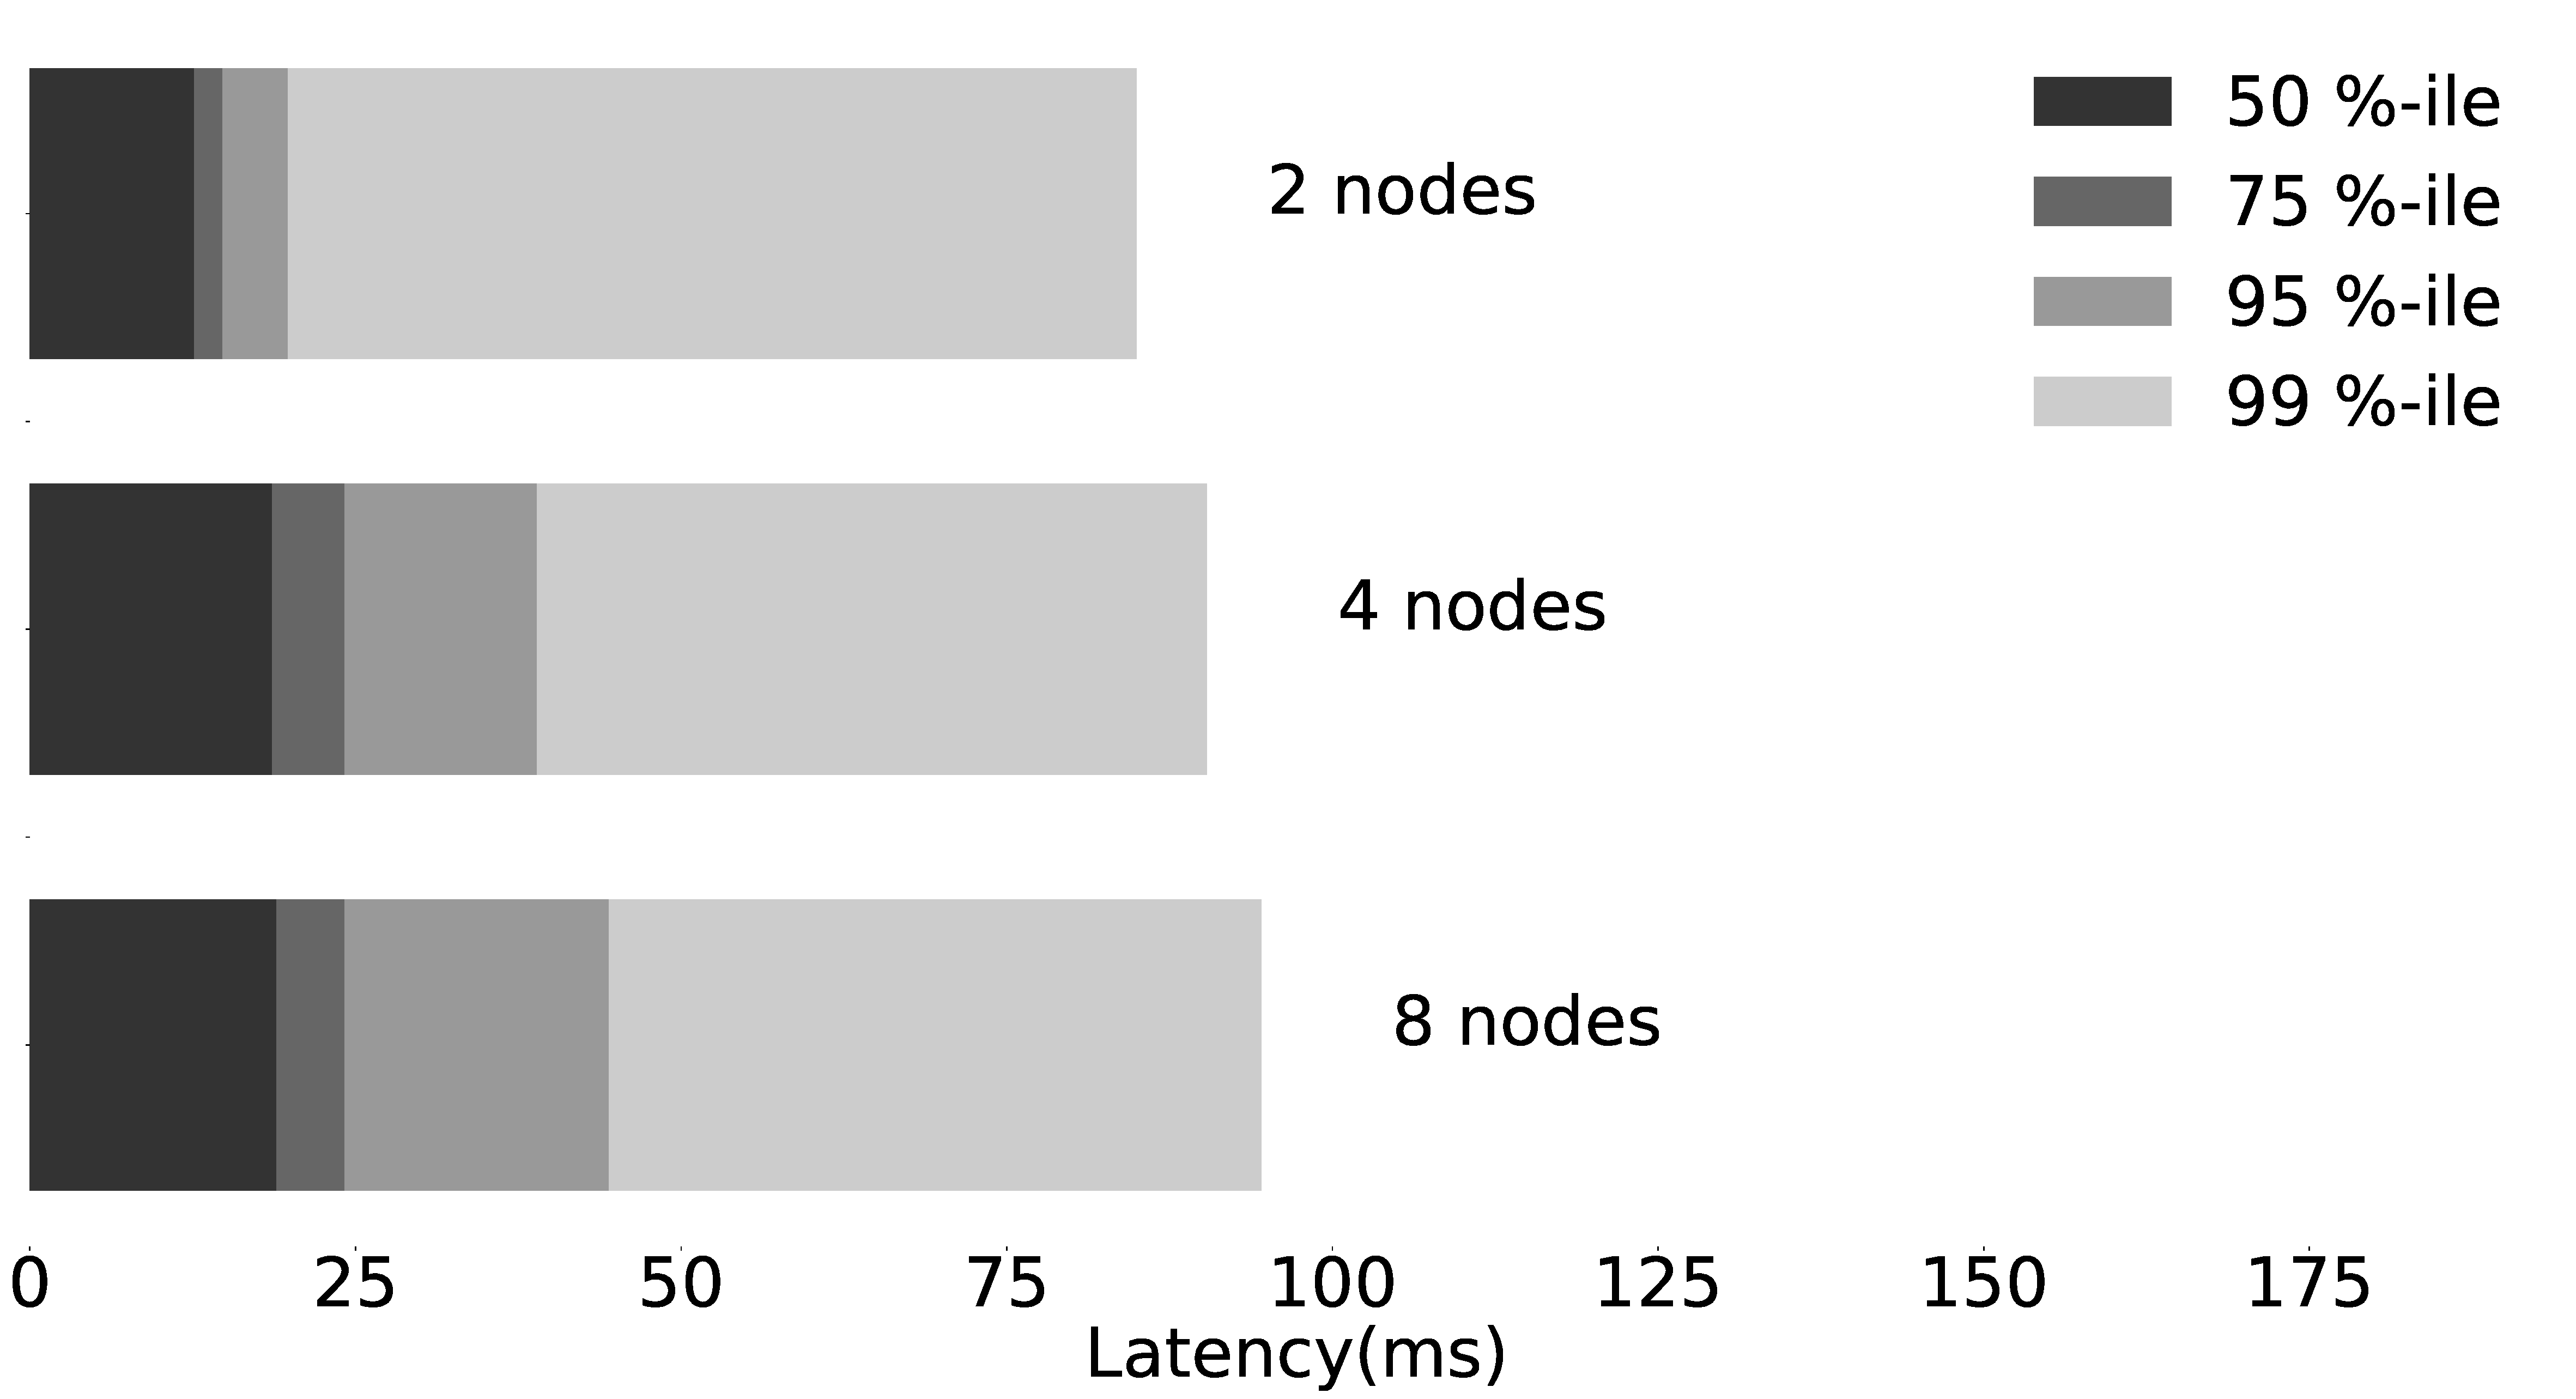
\includegraphics[scale=0.1]{pics/classifier_latencies}
  \caption{Prediction pipeline latencies}
  \label {latencies}
\end{figure}

\subsection{Data flow evaluation}

For evaluation, we deployed FlameStream on clusters, containing 2, 4 and 8 Amazon EC2 small instances with 2 GB of RAM and 1 core CPU. Exactly once guarantee was enabled. We measured throughput that is possible to achieve and the corresponding latency for prediction pipeline\footnote{We took into consideration only the performance of the streaming pipeline without a persistent queue}. The results are shown in Figures~\ref{latencies} and~\ref{throughput}. As we can see, there is a linear trend in throughput, which proves the scalability of the framework. On the other hand, one can observe, that latency increases moderately and keeps under 25 ms for a median and under 100 ms for 99th percentile.

\begin{figure}[htbp]
  \centering
  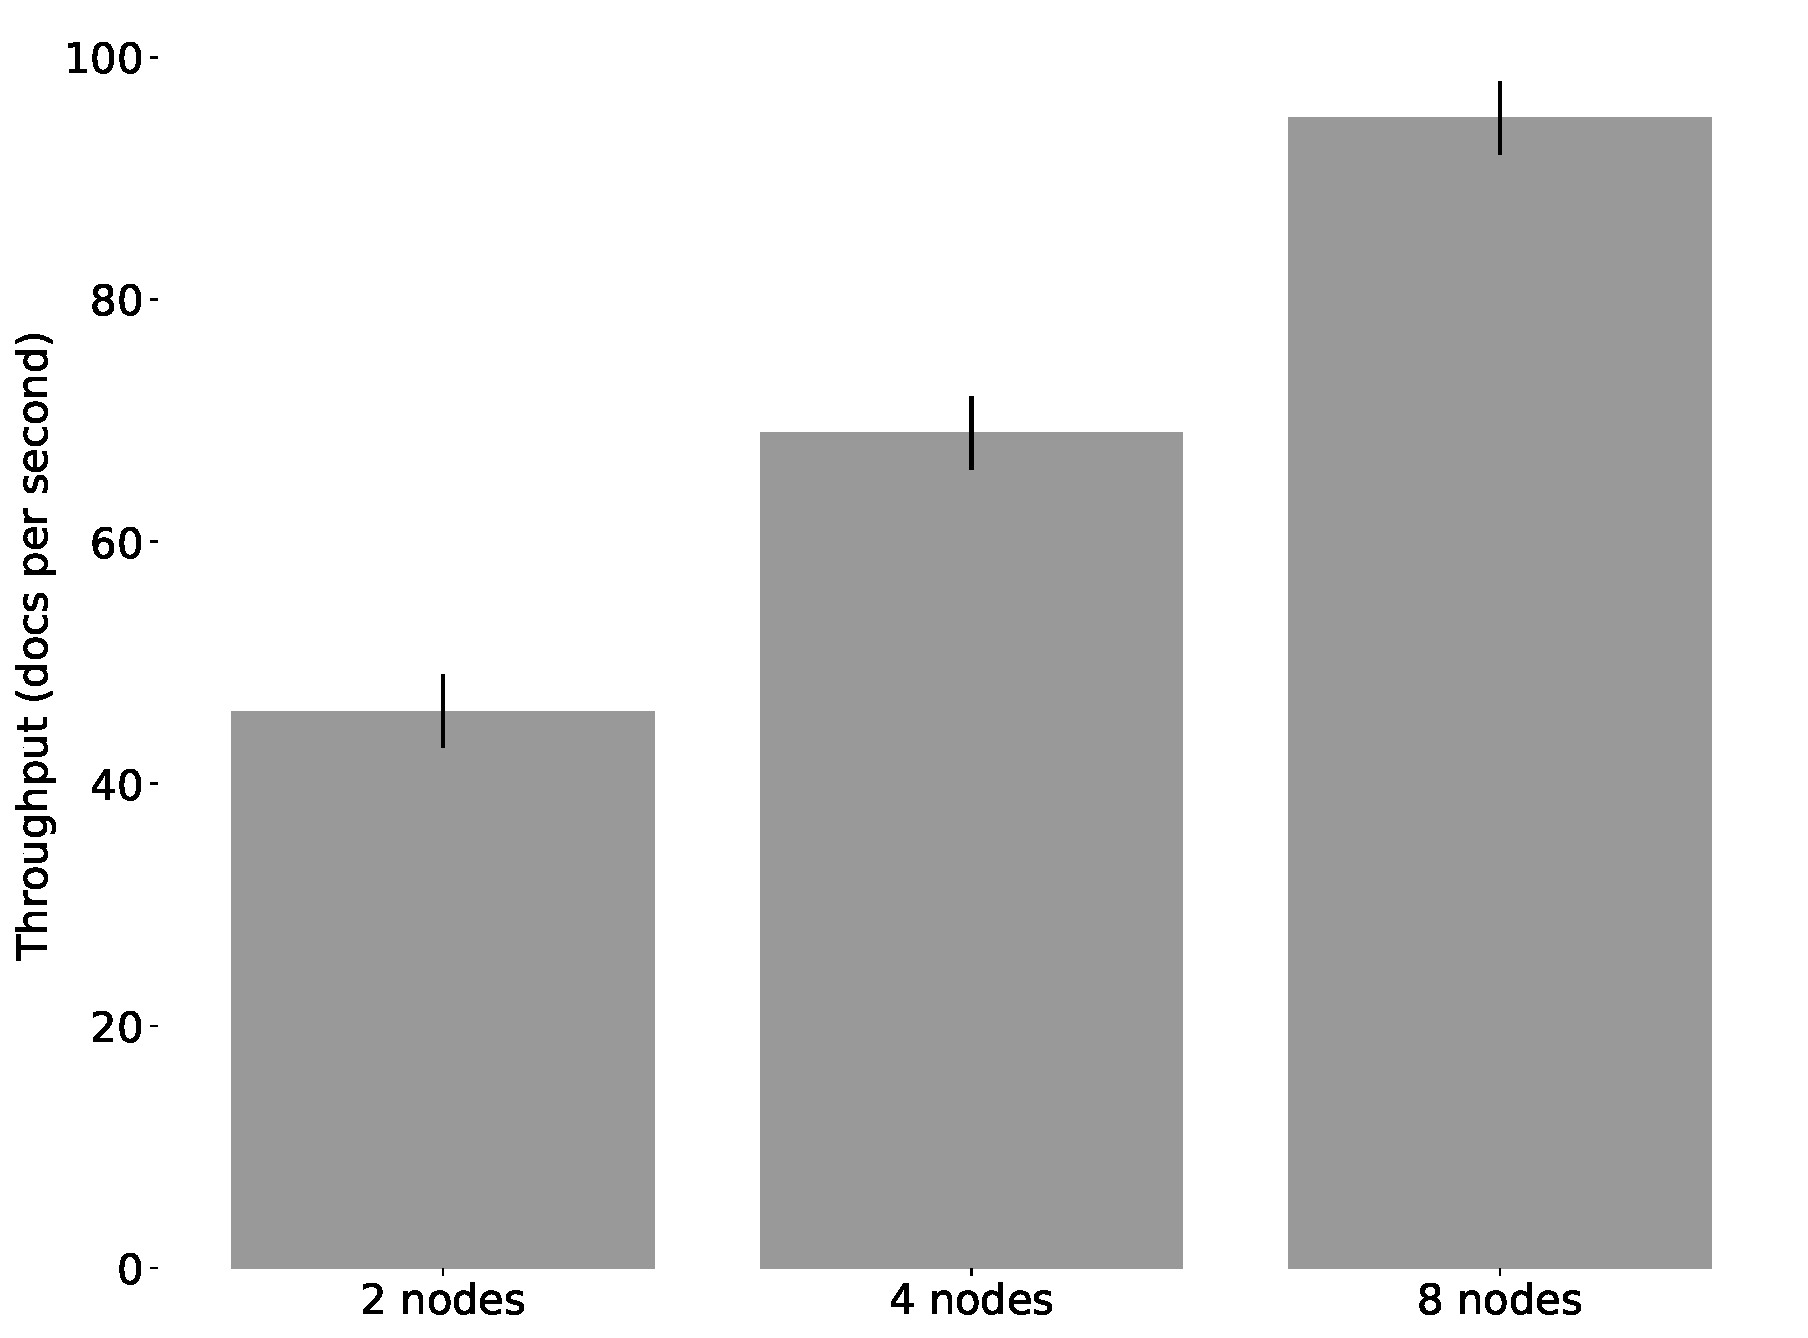
\includegraphics[scale=0.21]{pics/classifier_throughput}
  \caption{Prediction pipeline throughput}
  \label {throughput}
\end{figure}

\subsection{Classifier evaluation}

In order to be efficiently embedded in the proposed data flow, several properties of the machine learning model are desirable:
\begin{itemize}
     \item Small size of the model for storing and updating it in reasonable time and space.
     \item A possibility to update the model with new data.
\end{itemize}

We use Multinomial Logistic Regression as a classification method. Model parameters (weights) are denoted as $W$. The training process is the maximization of the following formula in terms of $W$:

$$ 
\begin{array}{rcl}
\log P(W | X)   & = &
 \frac 
      {1}{|X|} \sum \limits_{(x, y) \in X} \log \frac{e^{{W_y^T \cdot \; x}}}
      {\sum \limits_{l = 1}^{k}  e^{{W_{l}^T \cdot \; x}}}                  \\
  & & - \lambda_1 \parallel  W\parallel _1 
   - \lambda_2 \parallel  W - W_{prev} \parallel _2 
   \end {array}
   $$ 

$X$ denoted as a training dataset and the number of classes is $k$. Also, $x$ designated as a point in the dataset and $y$ as a label for it. To change the model over time, we use weights that are computed in the previous step -- $W_{prev}$. At the first step, $W_{prev}$ can be provided by a pre-train process.

The first component is the standard softmax function for multiple classes. The second component keeps the $L1$ regularization of the weights, and provides sparsity: with the dictionary of size 560 000, there is only 2\% of non-zero elements in $W$. Hence, the model has a small size -- about 10 Mb. We apply $L2$ regularization as the third component in order to use previous weights for on-the-fly model update.

We compared two approaches to the performance evaluation of the proposed machine learning model. The first one is training on the complete dataset with $\lambda_2 = 0$. We call this approach a {\em static training}. The second one consists in dividing training dataset into relatively small batches and consequent applying MLR with $L2$ regularization to each batch. The latter case demonstrates the behavior of our streaming classification approach. Dividing into train and test samples must be done uniformly in time in order to fairly evaluate streaming classifier. We calculate a hash function that depends on an input text to determine the use of text either in training or in the test sample. The sizes of the train and test sets are 50 000 and 100 000. The size of batches for the streaming approach is 5 000.

As one can see in Table~\ref{accuracy}, the streaming approach has a slightly lower accuracy in comparison with the static. The achieved value is reasonable considering the number of classes. These results indicate that our framework is able to efficiently solve the text multi-classification problem.

\begin{table}[htbp]
\caption{Accuracy comparison between static and stream training}
\begin{tabular}{lc}
Method             & Accuracy \% \\
Static training    & 0.609       \\
Streaming training & 0.601         
\end{tabular}
\label{accuracy}
\vspace{-7mm}
\end{table}

\section{Related Work}


Most related prior works were implemented on Apache Spark \cite{semberecki2016distributed} \cite{8029336} \cite{Nodarakis2016LargeSS} \cite{baltas2016apache} \cite{svyatkovskiy2016large} or Apache Storm \cite{khumoyun2016real}. These platforms use micro-batching technique for processing data. However, such method provides high latency between obtaining a text and labelling it. In addition, all the methods above does not consider a concept drift as an issue.

Next work takes into account the concept drift and related to stream data nature \cite{zhang2008one}. However, the final solution is hard to scale into a cluster of machines efficiently.

\section {Conclusion}
\label {fs-conclusion}

In this work, we investigated the suitability of distributed stream processing engines to the problem of text streams classification. We demonstrated that there are several pitfalls with an adaptation of data flow commonly used in batch systems for a stream processing:

\begin{itemize}
    \item Races in a physical data flow lead to irreproducible results: labels provided by a classifier may vary from run to run on the same test data. 
    \item Failures within {\em at least once} delivery guarantee can cause a biased distribution of classification results.
    \item Streaming data is rapidly changing, so there is a need to update the machine learning model on-the-fly. 
\end{itemize}

It was shown that straightforward solutions to the mentioned issues imply significant performance overhead. There were proposed potential solutions: to use~\FlameStream\ processing system with built-in determinism and efficient exactly once and to embed online learning into the data flow. 

As future work, we plan to implement a text classification framework that satisfies the following requirements:

\begin{itemize}
    \item Unbiased by distributed environment: node failures or races do not affect the ultimate result distribution.
    \item Reproducible: if input elements are stored in persistent storage, the same predictions are obtained on each new run.
    \item Concept drift conscious: changes in streaming data must be reflected in a machine learning model.  
\end{itemize}

\bibliographystyle{ACM-Reference-Format}
\bibliography{../../bibliography/flame-stream}

\end {document}

\endinput
